\documentclass[twoside]{book}

% Packages required by doxygen
\usepackage{fixltx2e}
\usepackage{calc}
\usepackage{doxygen}
\usepackage[export]{adjustbox} % also loads graphicx
\usepackage{graphicx}
\usepackage[utf8]{inputenc}
\usepackage{makeidx}
\usepackage{multicol}
\usepackage{multirow}
\PassOptionsToPackage{warn}{textcomp}
\usepackage{textcomp}
\usepackage[nointegrals]{wasysym}
\usepackage[table]{xcolor}

% Font selection
\usepackage[T1]{fontenc}
\usepackage[scaled=.90]{helvet}
\usepackage{courier}
\usepackage{amssymb}
\usepackage{sectsty}
\renewcommand{\familydefault}{\sfdefault}
\allsectionsfont{%
  \fontseries{bc}\selectfont%
  \color{darkgray}%
}
\renewcommand{\DoxyLabelFont}{%
  \fontseries{bc}\selectfont%
  \color{darkgray}%
}
\newcommand{\+}{\discretionary{\mbox{\scriptsize$\hookleftarrow$}}{}{}}

% Page & text layout
\usepackage{geometry}
\geometry{%
  a4paper,%
  top=2.5cm,%
  bottom=2.5cm,%
  left=2.5cm,%
  right=2.5cm%
}
\tolerance=750
\hfuzz=15pt
\hbadness=750
\setlength{\emergencystretch}{15pt}
\setlength{\parindent}{0cm}
\setlength{\parskip}{3ex plus 2ex minus 2ex}
\makeatletter
\renewcommand{\paragraph}{%
  \@startsection{paragraph}{4}{0ex}{-1.0ex}{1.0ex}{%
    \normalfont\normalsize\bfseries\SS@parafont%
  }%
}
\renewcommand{\subparagraph}{%
  \@startsection{subparagraph}{5}{0ex}{-1.0ex}{1.0ex}{%
    \normalfont\normalsize\bfseries\SS@subparafont%
  }%
}
\makeatother

% Headers & footers
\usepackage{fancyhdr}
\pagestyle{fancyplain}
\fancyhead[LE]{\fancyplain{}{\bfseries\thepage}}
\fancyhead[CE]{\fancyplain{}{}}
\fancyhead[RE]{\fancyplain{}{\bfseries\leftmark}}
\fancyhead[LO]{\fancyplain{}{\bfseries\rightmark}}
\fancyhead[CO]{\fancyplain{}{}}
\fancyhead[RO]{\fancyplain{}{\bfseries\thepage}}
\fancyfoot[LE]{\fancyplain{}{}}
\fancyfoot[CE]{\fancyplain{}{}}
\fancyfoot[RE]{\fancyplain{}{\bfseries\scriptsize Generated by Doxygen }}
\fancyfoot[LO]{\fancyplain{}{\bfseries\scriptsize Generated by Doxygen }}
\fancyfoot[CO]{\fancyplain{}{}}
\fancyfoot[RO]{\fancyplain{}{}}
\renewcommand{\footrulewidth}{0.4pt}
\renewcommand{\chaptermark}[1]{%
  \markboth{#1}{}%
}
\renewcommand{\sectionmark}[1]{%
  \markright{\thesection\ #1}%
}

% Indices & bibliography
\usepackage{natbib}
\usepackage[titles]{tocloft}
\setcounter{tocdepth}{3}
\setcounter{secnumdepth}{5}
\makeindex

% Hyperlinks (required, but should be loaded last)
\usepackage{ifpdf}
\ifpdf
  \usepackage[pdftex,pagebackref=true]{hyperref}
\else
  \usepackage[ps2pdf,pagebackref=true]{hyperref}
\fi
\hypersetup{%
  colorlinks=true,%
  linkcolor=blue,%
  citecolor=blue,%
  unicode%
}

% Custom commands
\newcommand{\clearemptydoublepage}{%
  \newpage{\pagestyle{empty}\cleardoublepage}%
}

\usepackage{caption}
\captionsetup{labelsep=space,justification=centering,font={bf},singlelinecheck=off,skip=4pt,position=top}

%===== C O N T E N T S =====

\begin{document}

% Titlepage & ToC
\hypersetup{pageanchor=false,
             bookmarksnumbered=true,
             pdfencoding=unicode
            }
\pagenumbering{roman}
\begin{titlepage}
\vspace*{7cm}
\begin{center}%
{\Large My Project }\\
\vspace*{1cm}
{\large Generated by Doxygen 1.8.11}\\
\end{center}
\end{titlepage}
\clearemptydoublepage
\tableofcontents
\clearemptydoublepage
\pagenumbering{arabic}
\hypersetup{pageanchor=true}

%--- Begin generated contents ---
\chapter{Class Index}
\section{Class List}
Here are the classes, structs, unions and interfaces with brief descriptions\+:\begin{DoxyCompactList}
\item\contentsline{section}{\hyperlink{structnode}{node} }{\pageref{structnode}}{}
\item\contentsline{section}{\hyperlink{structnode1}{node1} }{\pageref{structnode1}}{}
\item\contentsline{section}{\hyperlink{structnode__info}{node\+\_\+info} }{\pageref{structnode__info}}{}
\end{DoxyCompactList}

\chapter{File Index}
\section{File List}
Here is a list of all files with brief descriptions\+:\begin{DoxyCompactList}
\item\contentsline{section}{\hyperlink{Lab1_8c}{Lab1.\+c} }{\pageref{Lab1_8c}}{}
\end{DoxyCompactList}

\chapter{Class Documentation}
\hypertarget{structcorners}{}\section{corners Struct Reference}
\label{structcorners}\index{corners@{corners}}
\subsection*{Public Attributes}
\begin{DoxyCompactItemize}
\item 
int \hyperlink{structcorners_ad77606f823737fc1f1347b25e905c1a7}{ra}
\item 
int \hyperlink{structcorners_ad19782e14b4b905dd685ce98fe6e718a}{rb}
\item 
int \hyperlink{structcorners_a251b43b5ccbc55556b61ac665e9c6a6c}{ca}
\item 
int \hyperlink{structcorners_a9ce755b65013cb6bb59e4bd4c44878aa}{cb}
\end{DoxyCompactItemize}


\subsection{Member Data Documentation}
\index{corners@{corners}!ca@{ca}}
\index{ca@{ca}!corners@{corners}}
\subsubsection[{\texorpdfstring{ca}{ca}}]{\setlength{\rightskip}{0pt plus 5cm}int corners\+::ca}\hypertarget{structcorners_a251b43b5ccbc55556b61ac665e9c6a6c}{}\label{structcorners_a251b43b5ccbc55556b61ac665e9c6a6c}
\index{corners@{corners}!cb@{cb}}
\index{cb@{cb}!corners@{corners}}
\subsubsection[{\texorpdfstring{cb}{cb}}]{\setlength{\rightskip}{0pt plus 5cm}int corners\+::cb}\hypertarget{structcorners_a9ce755b65013cb6bb59e4bd4c44878aa}{}\label{structcorners_a9ce755b65013cb6bb59e4bd4c44878aa}
\index{corners@{corners}!ra@{ra}}
\index{ra@{ra}!corners@{corners}}
\subsubsection[{\texorpdfstring{ra}{ra}}]{\setlength{\rightskip}{0pt plus 5cm}int corners\+::ra}\hypertarget{structcorners_ad77606f823737fc1f1347b25e905c1a7}{}\label{structcorners_ad77606f823737fc1f1347b25e905c1a7}
\index{corners@{corners}!rb@{rb}}
\index{rb@{rb}!corners@{corners}}
\subsubsection[{\texorpdfstring{rb}{rb}}]{\setlength{\rightskip}{0pt plus 5cm}int corners\+::rb}\hypertarget{structcorners_ad19782e14b4b905dd685ce98fe6e718a}{}\label{structcorners_ad19782e14b4b905dd685ce98fe6e718a}


The documentation for this struct was generated from the following file\+:\begin{DoxyCompactItemize}
\item 
\hyperlink{Strassen_8cpp}{Strassen.\+cpp}\end{DoxyCompactItemize}

\chapter{File Documentation}
\hypertarget{Strassen_8cpp}{}\section{Strassen.\+cpp File Reference}
\label{Strassen_8cpp}\index{Strassen.\+cpp@{Strassen.\+cpp}}
{\ttfamily \#include $<$assert.\+h$>$}\\*
{\ttfamily \#include $<$stdio.\+h$>$}\\*
{\ttfamily \#include $<$stdlib.\+h$>$}\\*
{\ttfamily \#include $<$time.\+h$>$}\\*
Include dependency graph for Strassen.\+cpp\+:
\nopagebreak
\begin{figure}[H]
\begin{center}
\leavevmode
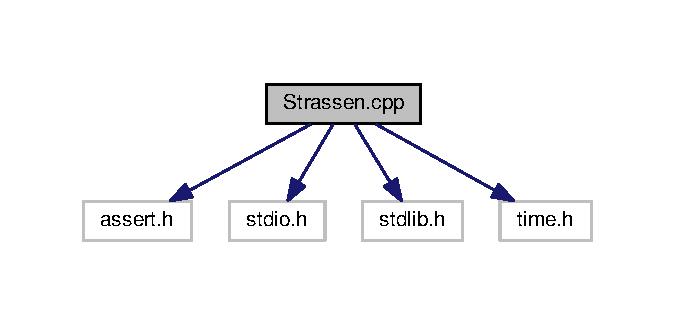
\includegraphics[width=324pt]{Strassen_8cpp__incl}
\end{center}
\end{figure}
\subsection*{Classes}
\begin{DoxyCompactItemize}
\item 
struct \hyperlink{structcorners}{corners}
\end{DoxyCompactItemize}
\subsection*{Macros}
\begin{DoxyCompactItemize}
\item 
\#define \hyperlink{Strassen_8cpp_a52037c938e3c1b126c6277da5ca689d0}{M}~2
\item 
\#define \hyperlink{Strassen_8cpp_a0240ac851181b84ac374872dc5434ee4}{N}~(1$<$$<$\hyperlink{Strassen_8cpp_a52037c938e3c1b126c6277da5ca689d0}{M})
\item 
\#define \hyperlink{Strassen_8cpp_a4bc1f413e2375a5a861ac19833775afc}{D\+A\+T\+A\+T\+Y\+P\+E\+\_\+\+F\+O\+R\+M\+AT}~\char`\"{}\%4.\+2g\char`\"{}
\item 
\#define \hyperlink{Strassen_8cpp_a63dd1f5e3e882f39ab54da1207031568}{L\+EN}(A)~(sizeof(A)/sizeof(A\mbox{[}0\mbox{]}))
\item 
\#define \hyperlink{Strassen_8cpp_a4e84a25ad27c37aa46c10622acf65777}{S\+T0}~\hyperlink{Strassen_8cpp_a6153ce67ed496c24db8c0c42c3d137f7}{set}(S,p,0); \hyperlink{Strassen_8cpp_a6153ce67ed496c24db8c0c42c3d137f7}{set}(T,p,0)
\end{DoxyCompactItemize}
\subsection*{Typedefs}
\begin{DoxyCompactItemize}
\item 
typedef double \hyperlink{Strassen_8cpp_a446c60693d6fa4c984642108301edc39}{datatype}
\item 
typedef \hyperlink{Strassen_8cpp_a446c60693d6fa4c984642108301edc39}{datatype} \hyperlink{Strassen_8cpp_a8efbe100dbea2d938eee767c887b461b}{mat}\mbox{[}\hyperlink{Strassen_8cpp_a0240ac851181b84ac374872dc5434ee4}{N}\mbox{]}\mbox{[}\hyperlink{Strassen_8cpp_a0240ac851181b84ac374872dc5434ee4}{N}\mbox{]}
\end{DoxyCompactItemize}
\subsection*{Functions}
\begin{DoxyCompactItemize}
\item 
void \hyperlink{Strassen_8cpp_aa65f3baa459cd757d47277dc83d35484}{identity} (\hyperlink{Strassen_8cpp_a8efbe100dbea2d938eee767c887b461b}{mat} A, \hyperlink{structcorners}{corners} a)
\item 
void \hyperlink{Strassen_8cpp_a6153ce67ed496c24db8c0c42c3d137f7}{set} (\hyperlink{Strassen_8cpp_a8efbe100dbea2d938eee767c887b461b}{mat} A, \hyperlink{structcorners}{corners} a, \hyperlink{Strassen_8cpp_a446c60693d6fa4c984642108301edc39}{datatype} k)
\item 
void \hyperlink{Strassen_8cpp_a3967885010fddda281509003e4b6d44b}{randk} (\hyperlink{Strassen_8cpp_a8efbe100dbea2d938eee767c887b461b}{mat} A, \hyperlink{structcorners}{corners} a, double l, double h)
\item 
void \hyperlink{Strassen_8cpp_a0a9af5da65ff575ce4423b5c517b1630}{print} (\hyperlink{Strassen_8cpp_a8efbe100dbea2d938eee767c887b461b}{mat} A, \hyperlink{structcorners}{corners} a, char $\ast$name)
\item 
void \hyperlink{Strassen_8cpp_a647e3a5e4e5a7eb64b3b56c1f62c44ca}{add} (\hyperlink{Strassen_8cpp_a8efbe100dbea2d938eee767c887b461b}{mat} A, \hyperlink{Strassen_8cpp_a8efbe100dbea2d938eee767c887b461b}{mat} B, \hyperlink{Strassen_8cpp_a8efbe100dbea2d938eee767c887b461b}{mat} C, \hyperlink{structcorners}{corners} a, \hyperlink{structcorners}{corners} b, \hyperlink{structcorners}{corners} c)
\item 
void \hyperlink{Strassen_8cpp_abcff7c86f333055c63829c0079479eab}{sub} (\hyperlink{Strassen_8cpp_a8efbe100dbea2d938eee767c887b461b}{mat} A, \hyperlink{Strassen_8cpp_a8efbe100dbea2d938eee767c887b461b}{mat} B, \hyperlink{Strassen_8cpp_a8efbe100dbea2d938eee767c887b461b}{mat} C, \hyperlink{structcorners}{corners} a, \hyperlink{structcorners}{corners} b, \hyperlink{structcorners}{corners} c)
\item 
void \hyperlink{Strassen_8cpp_a5a2b10f452cae73b4f00d593c96ce751}{find\+\_\+corner} (\hyperlink{structcorners}{corners} a, int i, int j, \hyperlink{structcorners}{corners} $\ast$b)
\item 
void \hyperlink{Strassen_8cpp_a3ea2ea8a59eedc6621a3e36ee422c379}{mul} (\hyperlink{Strassen_8cpp_a8efbe100dbea2d938eee767c887b461b}{mat} A, \hyperlink{Strassen_8cpp_a8efbe100dbea2d938eee767c887b461b}{mat} B, \hyperlink{Strassen_8cpp_a8efbe100dbea2d938eee767c887b461b}{mat} C, \hyperlink{structcorners}{corners} a, \hyperlink{structcorners}{corners} b, \hyperlink{structcorners}{corners} c)
\item 
int \hyperlink{Strassen_8cpp_ae66f6b31b5ad750f1fe042a706a4e3d4}{main} ()
\end{DoxyCompactItemize}


\subsection{Macro Definition Documentation}
\index{Strassen.\+cpp@{Strassen.\+cpp}!D\+A\+T\+A\+T\+Y\+P\+E\+\_\+\+F\+O\+R\+M\+AT@{D\+A\+T\+A\+T\+Y\+P\+E\+\_\+\+F\+O\+R\+M\+AT}}
\index{D\+A\+T\+A\+T\+Y\+P\+E\+\_\+\+F\+O\+R\+M\+AT@{D\+A\+T\+A\+T\+Y\+P\+E\+\_\+\+F\+O\+R\+M\+AT}!Strassen.\+cpp@{Strassen.\+cpp}}
\subsubsection[{\texorpdfstring{D\+A\+T\+A\+T\+Y\+P\+E\+\_\+\+F\+O\+R\+M\+AT}{DATATYPE_FORMAT}}]{\setlength{\rightskip}{0pt plus 5cm}\#define D\+A\+T\+A\+T\+Y\+P\+E\+\_\+\+F\+O\+R\+M\+AT~\char`\"{}\%4.\+2g\char`\"{}}\hypertarget{Strassen_8cpp_a4bc1f413e2375a5a861ac19833775afc}{}\label{Strassen_8cpp_a4bc1f413e2375a5a861ac19833775afc}
\index{Strassen.\+cpp@{Strassen.\+cpp}!L\+EN@{L\+EN}}
\index{L\+EN@{L\+EN}!Strassen.\+cpp@{Strassen.\+cpp}}
\subsubsection[{\texorpdfstring{L\+EN}{LEN}}]{\setlength{\rightskip}{0pt plus 5cm}\#define L\+EN(
\begin{DoxyParamCaption}
\item[{}]{A}
\end{DoxyParamCaption}
)~(sizeof(A)/sizeof(A\mbox{[}0\mbox{]}))}\hypertarget{Strassen_8cpp_a63dd1f5e3e882f39ab54da1207031568}{}\label{Strassen_8cpp_a63dd1f5e3e882f39ab54da1207031568}
\index{Strassen.\+cpp@{Strassen.\+cpp}!M@{M}}
\index{M@{M}!Strassen.\+cpp@{Strassen.\+cpp}}
\subsubsection[{\texorpdfstring{M}{M}}]{\setlength{\rightskip}{0pt plus 5cm}\#define M~2}\hypertarget{Strassen_8cpp_a52037c938e3c1b126c6277da5ca689d0}{}\label{Strassen_8cpp_a52037c938e3c1b126c6277da5ca689d0}
\index{Strassen.\+cpp@{Strassen.\+cpp}!N@{N}}
\index{N@{N}!Strassen.\+cpp@{Strassen.\+cpp}}
\subsubsection[{\texorpdfstring{N}{N}}]{\setlength{\rightskip}{0pt plus 5cm}\#define N~(1$<$$<${\bf M})}\hypertarget{Strassen_8cpp_a0240ac851181b84ac374872dc5434ee4}{}\label{Strassen_8cpp_a0240ac851181b84ac374872dc5434ee4}
\index{Strassen.\+cpp@{Strassen.\+cpp}!S\+T0@{S\+T0}}
\index{S\+T0@{S\+T0}!Strassen.\+cpp@{Strassen.\+cpp}}
\subsubsection[{\texorpdfstring{S\+T0}{ST0}}]{\setlength{\rightskip}{0pt plus 5cm}\#define S\+T0~{\bf set}(S,p,0); {\bf set}(T,p,0)}\hypertarget{Strassen_8cpp_a4e84a25ad27c37aa46c10622acf65777}{}\label{Strassen_8cpp_a4e84a25ad27c37aa46c10622acf65777}


\subsection{Typedef Documentation}
\index{Strassen.\+cpp@{Strassen.\+cpp}!datatype@{datatype}}
\index{datatype@{datatype}!Strassen.\+cpp@{Strassen.\+cpp}}
\subsubsection[{\texorpdfstring{datatype}{datatype}}]{\setlength{\rightskip}{0pt plus 5cm}typedef double {\bf datatype}}\hypertarget{Strassen_8cpp_a446c60693d6fa4c984642108301edc39}{}\label{Strassen_8cpp_a446c60693d6fa4c984642108301edc39}
\index{Strassen.\+cpp@{Strassen.\+cpp}!mat@{mat}}
\index{mat@{mat}!Strassen.\+cpp@{Strassen.\+cpp}}
\subsubsection[{\texorpdfstring{mat}{mat}}]{\setlength{\rightskip}{0pt plus 5cm}typedef {\bf datatype} mat\mbox{[}{\bf N}\mbox{]}\mbox{[}{\bf N}\mbox{]}}\hypertarget{Strassen_8cpp_a8efbe100dbea2d938eee767c887b461b}{}\label{Strassen_8cpp_a8efbe100dbea2d938eee767c887b461b}


\subsection{Function Documentation}
\index{Strassen.\+cpp@{Strassen.\+cpp}!add@{add}}
\index{add@{add}!Strassen.\+cpp@{Strassen.\+cpp}}
\subsubsection[{\texorpdfstring{add(mat A, mat B, mat C, corners a, corners b, corners c)}{add(mat A, mat B, mat C, corners a, corners b, corners c)}}]{\setlength{\rightskip}{0pt plus 5cm}void add (
\begin{DoxyParamCaption}
\item[{{\bf mat}}]{A, }
\item[{{\bf mat}}]{B, }
\item[{{\bf mat}}]{C, }
\item[{{\bf corners}}]{a, }
\item[{{\bf corners}}]{b, }
\item[{{\bf corners}}]{c}
\end{DoxyParamCaption}
)}\hypertarget{Strassen_8cpp_a647e3a5e4e5a7eb64b3b56c1f62c44ca}{}\label{Strassen_8cpp_a647e3a5e4e5a7eb64b3b56c1f62c44ca}

\begin{DoxyCode}
61 \{
62     \textcolor{keywordtype}{int} rd = a.\hyperlink{structcorners_ad19782e14b4b905dd685ce98fe6e718a}{rb} - a.\hyperlink{structcorners_ad77606f823737fc1f1347b25e905c1a7}{ra};
63     \textcolor{keywordtype}{int} cd = a.\hyperlink{structcorners_a9ce755b65013cb6bb59e4bd4c44878aa}{cb} - a.\hyperlink{structcorners_a251b43b5ccbc55556b61ac665e9c6a6c}{ca};
64     \textcolor{keywordtype}{int} i, j;
65     \textcolor{keywordflow}{for} (i = 0; i < rd; i++)
66     \{
67         \textcolor{keywordflow}{for} (j = 0; j < cd; j++)
68         \{
69             C[i + c.\hyperlink{structcorners_ad77606f823737fc1f1347b25e905c1a7}{ra}][j + c.\hyperlink{structcorners_a251b43b5ccbc55556b61ac665e9c6a6c}{ca}] = A[i + a.\hyperlink{structcorners_ad77606f823737fc1f1347b25e905c1a7}{ra}][j + a.\hyperlink{structcorners_a251b43b5ccbc55556b61ac665e9c6a6c}{ca}] + B[i + b.\hyperlink{structcorners_ad77606f823737fc1f1347b25e905c1a7}{ra}][j
70                     + b.\hyperlink{structcorners_a251b43b5ccbc55556b61ac665e9c6a6c}{ca}];
71         \}
72     \}
73 \}
\end{DoxyCode}
\index{Strassen.\+cpp@{Strassen.\+cpp}!find\+\_\+corner@{find\+\_\+corner}}
\index{find\+\_\+corner@{find\+\_\+corner}!Strassen.\+cpp@{Strassen.\+cpp}}
\subsubsection[{\texorpdfstring{find\+\_\+corner(corners a, int i, int j, corners $\ast$b)}{find_corner(corners a, int i, int j, corners *b)}}]{\setlength{\rightskip}{0pt plus 5cm}void find\+\_\+corner (
\begin{DoxyParamCaption}
\item[{{\bf corners}}]{a, }
\item[{int}]{i, }
\item[{int}]{j, }
\item[{{\bf corners} $\ast$}]{b}
\end{DoxyParamCaption}
)}\hypertarget{Strassen_8cpp_a5a2b10f452cae73b4f00d593c96ce751}{}\label{Strassen_8cpp_a5a2b10f452cae73b4f00d593c96ce751}

\begin{DoxyCode}
93 \{
94     \textcolor{keywordtype}{int} rm = a.\hyperlink{structcorners_ad77606f823737fc1f1347b25e905c1a7}{ra} + (a.\hyperlink{structcorners_ad19782e14b4b905dd685ce98fe6e718a}{rb} - a.\hyperlink{structcorners_ad77606f823737fc1f1347b25e905c1a7}{ra}) / 2;
95     \textcolor{keywordtype}{int} cm = a.\hyperlink{structcorners_a251b43b5ccbc55556b61ac665e9c6a6c}{ca} + (a.\hyperlink{structcorners_a9ce755b65013cb6bb59e4bd4c44878aa}{cb} - a.\hyperlink{structcorners_a251b43b5ccbc55556b61ac665e9c6a6c}{ca}) / 2;
96     *b = a;
97     \textcolor{keywordflow}{if} (i == 0)
98         b->\hyperlink{structcorners_ad19782e14b4b905dd685ce98fe6e718a}{rb} = rm; \textcolor{comment}{// top rows}
99     \textcolor{keywordflow}{else}
100         b->\hyperlink{structcorners_ad77606f823737fc1f1347b25e905c1a7}{ra} = rm; \textcolor{comment}{// bot rows}
101     \textcolor{keywordflow}{if} (j == 0)
102         b->\hyperlink{structcorners_a9ce755b65013cb6bb59e4bd4c44878aa}{cb} = cm; \textcolor{comment}{// left cols}
103     \textcolor{keywordflow}{else}
104         b->\hyperlink{structcorners_a251b43b5ccbc55556b61ac665e9c6a6c}{ca} = cm; \textcolor{comment}{// right cols}
105 \}
\end{DoxyCode}
\index{Strassen.\+cpp@{Strassen.\+cpp}!identity@{identity}}
\index{identity@{identity}!Strassen.\+cpp@{Strassen.\+cpp}}
\subsubsection[{\texorpdfstring{identity(mat A, corners a)}{identity(mat A, corners a)}}]{\setlength{\rightskip}{0pt plus 5cm}void identity (
\begin{DoxyParamCaption}
\item[{{\bf mat}}]{A, }
\item[{{\bf corners}}]{a}
\end{DoxyParamCaption}
)}\hypertarget{Strassen_8cpp_aa65f3baa459cd757d47277dc83d35484}{}\label{Strassen_8cpp_aa65f3baa459cd757d47277dc83d35484}

\begin{DoxyCode}
20 \{
21     \textcolor{keywordtype}{int} i, j;
22     \textcolor{keywordflow}{for} (i = a.\hyperlink{structcorners_ad77606f823737fc1f1347b25e905c1a7}{ra}; i < a.\hyperlink{structcorners_ad19782e14b4b905dd685ce98fe6e718a}{rb}; i++)
23         \textcolor{keywordflow}{for} (j = a.\hyperlink{structcorners_a251b43b5ccbc55556b61ac665e9c6a6c}{ca}; j < a.\hyperlink{structcorners_a9ce755b65013cb6bb59e4bd4c44878aa}{cb}; j++)
24             A[i][j] = (\hyperlink{Strassen_8cpp_a446c60693d6fa4c984642108301edc39}{datatype}) (i == j);
25 \}
\end{DoxyCode}
\index{Strassen.\+cpp@{Strassen.\+cpp}!main@{main}}
\index{main@{main}!Strassen.\+cpp@{Strassen.\+cpp}}
\subsubsection[{\texorpdfstring{main()}{main()}}]{\setlength{\rightskip}{0pt plus 5cm}int main (
\begin{DoxyParamCaption}
{}
\end{DoxyParamCaption}
)}\hypertarget{Strassen_8cpp_ae66f6b31b5ad750f1fe042a706a4e3d4}{}\label{Strassen_8cpp_ae66f6b31b5ad750f1fe042a706a4e3d4}

\begin{DoxyCode}
207 \{
208     \hyperlink{Strassen_8cpp_a8efbe100dbea2d938eee767c887b461b}{mat} A, B, C;
209     \hyperlink{structcorners}{corners} ai = \{ 0, \hyperlink{Strassen_8cpp_a0240ac851181b84ac374872dc5434ee4}{N}, 0, \hyperlink{Strassen_8cpp_a0240ac851181b84ac374872dc5434ee4}{N} \};
210     \hyperlink{structcorners}{corners} bi = \{ 0, \hyperlink{Strassen_8cpp_a0240ac851181b84ac374872dc5434ee4}{N}, 0, N \};
211     \hyperlink{structcorners}{corners} ci = \{ 0, \hyperlink{Strassen_8cpp_a0240ac851181b84ac374872dc5434ee4}{N}, 0, N \};
212     srand(time(0));
213     \textcolor{comment}{// identity(A,bi); identity(B,bi);}
214     \textcolor{comment}{// set(A,ai,2); set(B,bi,2);}
215     \hyperlink{Strassen_8cpp_a3967885010fddda281509003e4b6d44b}{randk}(A, ai, 0, 2);
216     \hyperlink{Strassen_8cpp_a3967885010fddda281509003e4b6d44b}{randk}(B, bi, 0, 2);
217     \hyperlink{Strassen_8cpp_a0a9af5da65ff575ce4423b5c517b1630}{print}(A, ai, \textcolor{stringliteral}{"A"});
218     \hyperlink{Strassen_8cpp_a0a9af5da65ff575ce4423b5c517b1630}{print}(B, bi, \textcolor{stringliteral}{"B"});
219     \textcolor{keyword}{set}(C, ci, 0);
220     \textcolor{comment}{// add(A,B,C, ai, bi, ci);}
221     \hyperlink{Strassen_8cpp_a3ea2ea8a59eedc6621a3e36ee422c379}{mul}(A, B, C, ai, bi, ci);
222     \hyperlink{Strassen_8cpp_a0a9af5da65ff575ce4423b5c517b1630}{print}(C, ci, \textcolor{stringliteral}{"C"});
223     \textcolor{keywordflow}{return} 0;
224 \}\end{DoxyCode}


Here is the call graph for this function\+:
\nopagebreak
\begin{figure}[H]
\begin{center}
\leavevmode
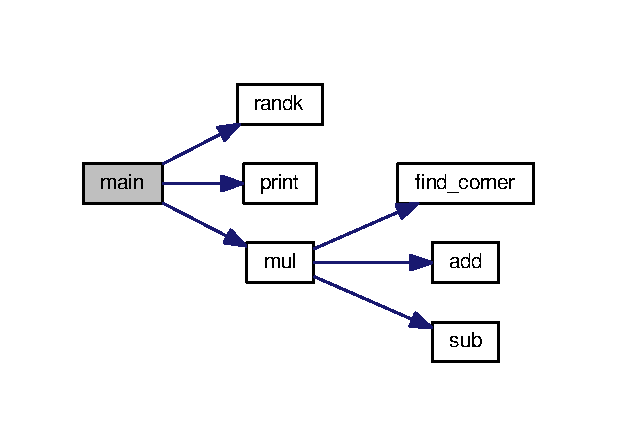
\includegraphics[width=296pt]{Strassen_8cpp_ae66f6b31b5ad750f1fe042a706a4e3d4_cgraph}
\end{center}
\end{figure}


\index{Strassen.\+cpp@{Strassen.\+cpp}!mul@{mul}}
\index{mul@{mul}!Strassen.\+cpp@{Strassen.\+cpp}}
\subsubsection[{\texorpdfstring{mul(mat A, mat B, mat C, corners a, corners b, corners c)}{mul(mat A, mat B, mat C, corners a, corners b, corners c)}}]{\setlength{\rightskip}{0pt plus 5cm}void mul (
\begin{DoxyParamCaption}
\item[{{\bf mat}}]{A, }
\item[{{\bf mat}}]{B, }
\item[{{\bf mat}}]{C, }
\item[{{\bf corners}}]{a, }
\item[{{\bf corners}}]{b, }
\item[{{\bf corners}}]{c}
\end{DoxyParamCaption}
)}\hypertarget{Strassen_8cpp_a3ea2ea8a59eedc6621a3e36ee422c379}{}\label{Strassen_8cpp_a3ea2ea8a59eedc6621a3e36ee422c379}

\begin{DoxyCode}
109 \{
110     \hyperlink{structcorners}{corners} aii[2][2], bii[2][2], cii[2][2], p;
111     \hyperlink{Strassen_8cpp_a8efbe100dbea2d938eee767c887b461b}{mat} P[7], S, T;
112     \textcolor{keywordtype}{int} i, j, m, n, k;
113  
114     \textcolor{comment}{// Check: A[m n] * B[n k] = C[m k]}
115     m = a.\hyperlink{structcorners_ad19782e14b4b905dd685ce98fe6e718a}{rb} - a.\hyperlink{structcorners_ad77606f823737fc1f1347b25e905c1a7}{ra};
116     assert(m==(c.\hyperlink{structcorners_ad19782e14b4b905dd685ce98fe6e718a}{rb}-c.\hyperlink{structcorners_ad77606f823737fc1f1347b25e905c1a7}{ra}));
117     n = a.\hyperlink{structcorners_a9ce755b65013cb6bb59e4bd4c44878aa}{cb} - a.\hyperlink{structcorners_a251b43b5ccbc55556b61ac665e9c6a6c}{ca};
118     assert(n==(b.\hyperlink{structcorners_ad19782e14b4b905dd685ce98fe6e718a}{rb}-b.\hyperlink{structcorners_ad77606f823737fc1f1347b25e905c1a7}{ra}));
119     k = b.\hyperlink{structcorners_a9ce755b65013cb6bb59e4bd4c44878aa}{cb} - b.\hyperlink{structcorners_a251b43b5ccbc55556b61ac665e9c6a6c}{ca};
120     assert(k==(c.\hyperlink{structcorners_a9ce755b65013cb6bb59e4bd4c44878aa}{cb}-c.\hyperlink{structcorners_a251b43b5ccbc55556b61ac665e9c6a6c}{ca}));
121     assert(m>0);
122  
123     \textcolor{keywordflow}{if} (n == 1)
124     \{
125         C[c.\hyperlink{structcorners_ad77606f823737fc1f1347b25e905c1a7}{ra}][c.\hyperlink{structcorners_a251b43b5ccbc55556b61ac665e9c6a6c}{ca}] += A[a.\hyperlink{structcorners_ad77606f823737fc1f1347b25e905c1a7}{ra}][a.\hyperlink{structcorners_a251b43b5ccbc55556b61ac665e9c6a6c}{ca}] * B[b.\hyperlink{structcorners_ad77606f823737fc1f1347b25e905c1a7}{ra}][b.\hyperlink{structcorners_a251b43b5ccbc55556b61ac665e9c6a6c}{ca}];
126         \textcolor{keywordflow}{return};
127     \}
128  
129     \textcolor{comment}{// Create the 12 smaller matrix indexes:}
130     \textcolor{comment}{//  A00 A01   B00 B01   C00 C01}
131     \textcolor{comment}{//  A10 A11   B10 B11   C10 C11}
132     \textcolor{keywordflow}{for} (i = 0; i < 2; i++)
133     \{
134         \textcolor{keywordflow}{for} (j = 0; j < 2; j++)
135         \{
136             \hyperlink{Strassen_8cpp_a5a2b10f452cae73b4f00d593c96ce751}{find\_corner}(a, i, j, &aii[i][j]);
137             \hyperlink{Strassen_8cpp_a5a2b10f452cae73b4f00d593c96ce751}{find\_corner}(b, i, j, &bii[i][j]);
138             \hyperlink{Strassen_8cpp_a5a2b10f452cae73b4f00d593c96ce751}{find\_corner}(c, i, j, &cii[i][j]);
139         \}
140     \}
141  
142     p.\hyperlink{structcorners_ad77606f823737fc1f1347b25e905c1a7}{ra} = p.\hyperlink{structcorners_a251b43b5ccbc55556b61ac665e9c6a6c}{ca} = 0;
143     p.\hyperlink{structcorners_ad19782e14b4b905dd685ce98fe6e718a}{rb} = p.\hyperlink{structcorners_a9ce755b65013cb6bb59e4bd4c44878aa}{cb} = m / 2;
144  
145 \textcolor{preprocessor}{#define LEN(A) (sizeof(A)/sizeof(A[0]))}
146     \textcolor{keywordflow}{for} (i = 0; i < \hyperlink{Strassen_8cpp_a63dd1f5e3e882f39ab54da1207031568}{LEN}(P); i++)
147         \textcolor{keyword}{set}(P[i], p, 0);
148  
149 \textcolor{preprocessor}{#define ST0 set(S,p,0); set(T,p,0)}
150  
151     \textcolor{comment}{// (A00 + A11) * (B00+B11) = S * T = P0}
152     \hyperlink{Strassen_8cpp_a4e84a25ad27c37aa46c10622acf65777}{ST0};
153     \hyperlink{Strassen_8cpp_a647e3a5e4e5a7eb64b3b56c1f62c44ca}{add}(A, A, S, aii[0][0], aii[1][1], p);
154     \hyperlink{Strassen_8cpp_a647e3a5e4e5a7eb64b3b56c1f62c44ca}{add}(B, B, T, bii[0][0], bii[1][1], p);
155     \hyperlink{Strassen_8cpp_a3ea2ea8a59eedc6621a3e36ee422c379}{mul}(S, T, P[0], p, p, p);
156  
157     \textcolor{comment}{// (A10 + A11) * B00 = S * B00 = P1}
158     \hyperlink{Strassen_8cpp_a4e84a25ad27c37aa46c10622acf65777}{ST0};
159     \hyperlink{Strassen_8cpp_a647e3a5e4e5a7eb64b3b56c1f62c44ca}{add}(A, A, S, aii[1][0], aii[1][1], p);
160     \hyperlink{Strassen_8cpp_a3ea2ea8a59eedc6621a3e36ee422c379}{mul}(S, B, P[1], p, bii[0][0], p);
161  
162     \textcolor{comment}{// A00 * (B01 - B11) = A00 * T = P2}
163     \hyperlink{Strassen_8cpp_a4e84a25ad27c37aa46c10622acf65777}{ST0};
164     \hyperlink{Strassen_8cpp_abcff7c86f333055c63829c0079479eab}{sub}(B, B, T, bii[0][1], bii[1][1], p);
165     \hyperlink{Strassen_8cpp_a3ea2ea8a59eedc6621a3e36ee422c379}{mul}(A, T, P[2], aii[0][0], p, p);
166  
167     \textcolor{comment}{// A11 * (B10 - B00) = A11 * T = P3}
168     \hyperlink{Strassen_8cpp_a4e84a25ad27c37aa46c10622acf65777}{ST0};
169     \hyperlink{Strassen_8cpp_abcff7c86f333055c63829c0079479eab}{sub}(B, B, T, bii[1][0], bii[0][0], p);
170     \hyperlink{Strassen_8cpp_a3ea2ea8a59eedc6621a3e36ee422c379}{mul}(A, T, P[3], aii[1][1], p, p);
171  
172     \textcolor{comment}{// (A00 + A01) * B11 = S * B11 = P4}
173     \hyperlink{Strassen_8cpp_a4e84a25ad27c37aa46c10622acf65777}{ST0};
174     \hyperlink{Strassen_8cpp_a647e3a5e4e5a7eb64b3b56c1f62c44ca}{add}(A, A, S, aii[0][0], aii[0][1], p);
175     \hyperlink{Strassen_8cpp_a3ea2ea8a59eedc6621a3e36ee422c379}{mul}(S, B, P[4], p, bii[1][1], p);
176  
177     \textcolor{comment}{// (A10 - A00) * (B00 + B01) = S * T = P5}
178     \hyperlink{Strassen_8cpp_a4e84a25ad27c37aa46c10622acf65777}{ST0};
179     \hyperlink{Strassen_8cpp_abcff7c86f333055c63829c0079479eab}{sub}(A, A, S, aii[1][0], aii[0][0], p);
180     \hyperlink{Strassen_8cpp_a647e3a5e4e5a7eb64b3b56c1f62c44ca}{add}(B, B, T, bii[0][0], bii[0][1], p);
181     \hyperlink{Strassen_8cpp_a3ea2ea8a59eedc6621a3e36ee422c379}{mul}(S, T, P[5], p, p, p);
182  
183     \textcolor{comment}{// (A01 - A11) * (B10 + B11) = S * T = P6}
184     \hyperlink{Strassen_8cpp_a4e84a25ad27c37aa46c10622acf65777}{ST0};
185     \hyperlink{Strassen_8cpp_abcff7c86f333055c63829c0079479eab}{sub}(A, A, S, aii[0][1], aii[1][1], p);
186     \hyperlink{Strassen_8cpp_a647e3a5e4e5a7eb64b3b56c1f62c44ca}{add}(B, B, T, bii[1][0], bii[1][1], p);
187     \hyperlink{Strassen_8cpp_a3ea2ea8a59eedc6621a3e36ee422c379}{mul}(S, T, P[6], p, p, p);
188  
189     \textcolor{comment}{// P0 + P3 - P4 + P6 = S - P4 + P6 = T + P6 = C00}
190     \hyperlink{Strassen_8cpp_a647e3a5e4e5a7eb64b3b56c1f62c44ca}{add}(P[0], P[3], S, p, p, p);
191     \hyperlink{Strassen_8cpp_abcff7c86f333055c63829c0079479eab}{sub}(S, P[4], T, p, p, p);
192     \hyperlink{Strassen_8cpp_a647e3a5e4e5a7eb64b3b56c1f62c44ca}{add}(T, P[6], C, p, p, cii[0][0]);
193  
194     \textcolor{comment}{// P2 + P4 = C01}
195     \hyperlink{Strassen_8cpp_a647e3a5e4e5a7eb64b3b56c1f62c44ca}{add}(P[2], P[4], C, p, p, cii[0][1]);
196  
197     \textcolor{comment}{// P1 + P3 = C10}
198     \hyperlink{Strassen_8cpp_a647e3a5e4e5a7eb64b3b56c1f62c44ca}{add}(P[1], P[3], C, p, p, cii[1][0]);
199  
200     \textcolor{comment}{// P0 + P2 - P1 + P5 = S - P1 + P5 = T + P5 = C11}
201     \hyperlink{Strassen_8cpp_a647e3a5e4e5a7eb64b3b56c1f62c44ca}{add}(P[0], P[2], S, p, p, p);
202     \hyperlink{Strassen_8cpp_abcff7c86f333055c63829c0079479eab}{sub}(S, P[1], T, p, p, p);
203     \hyperlink{Strassen_8cpp_a647e3a5e4e5a7eb64b3b56c1f62c44ca}{add}(T, P[5], C, p, p, cii[1][1]);
204  
205 \}
\end{DoxyCode}


Here is the call graph for this function\+:
\nopagebreak
\begin{figure}[H]
\begin{center}
\leavevmode
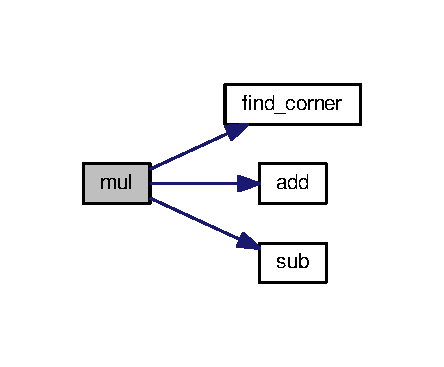
\includegraphics[width=213pt]{Strassen_8cpp_a3ea2ea8a59eedc6621a3e36ee422c379_cgraph}
\end{center}
\end{figure}


\index{Strassen.\+cpp@{Strassen.\+cpp}!print@{print}}
\index{print@{print}!Strassen.\+cpp@{Strassen.\+cpp}}
\subsubsection[{\texorpdfstring{print(mat A, corners a, char $\ast$name)}{print(mat A, corners a, char *name)}}]{\setlength{\rightskip}{0pt plus 5cm}void print (
\begin{DoxyParamCaption}
\item[{{\bf mat}}]{A, }
\item[{{\bf corners}}]{a, }
\item[{char $\ast$}]{name}
\end{DoxyParamCaption}
)}\hypertarget{Strassen_8cpp_a0a9af5da65ff575ce4423b5c517b1630}{}\label{Strassen_8cpp_a0a9af5da65ff575ce4423b5c517b1630}

\begin{DoxyCode}
47 \{
48     \textcolor{keywordtype}{int} i, j;
49     printf(\textcolor{stringliteral}{"%s = \{\(\backslash\)n"}, name);
50     \textcolor{keywordflow}{for} (i = a.\hyperlink{structcorners_ad77606f823737fc1f1347b25e905c1a7}{ra}; i < a.\hyperlink{structcorners_ad19782e14b4b905dd685ce98fe6e718a}{rb}; i++)
51     \{
52         \textcolor{keywordflow}{for} (j = a.\hyperlink{structcorners_a251b43b5ccbc55556b61ac665e9c6a6c}{ca}; j < a.\hyperlink{structcorners_a9ce755b65013cb6bb59e4bd4c44878aa}{cb}; j++)
53             printf(\hyperlink{Strassen_8cpp_a4bc1f413e2375a5a861ac19833775afc}{DATATYPE\_FORMAT} \textcolor{stringliteral}{", "}, A[i][j]);
54         printf(\textcolor{stringliteral}{"\(\backslash\)n"});
55     \}
56     printf(\textcolor{stringliteral}{"\}\(\backslash\)n"});
57 \}
\end{DoxyCode}
\index{Strassen.\+cpp@{Strassen.\+cpp}!randk@{randk}}
\index{randk@{randk}!Strassen.\+cpp@{Strassen.\+cpp}}
\subsubsection[{\texorpdfstring{randk(mat A, corners a, double l, double h)}{randk(mat A, corners a, double l, double h)}}]{\setlength{\rightskip}{0pt plus 5cm}void randk (
\begin{DoxyParamCaption}
\item[{{\bf mat}}]{A, }
\item[{{\bf corners}}]{a, }
\item[{double}]{l, }
\item[{double}]{h}
\end{DoxyParamCaption}
)}\hypertarget{Strassen_8cpp_a3967885010fddda281509003e4b6d44b}{}\label{Strassen_8cpp_a3967885010fddda281509003e4b6d44b}

\begin{DoxyCode}
38 \{
39     \textcolor{keywordtype}{int} i, j;
40     \textcolor{keywordflow}{for} (i = a.\hyperlink{structcorners_ad77606f823737fc1f1347b25e905c1a7}{ra}; i < a.\hyperlink{structcorners_ad19782e14b4b905dd685ce98fe6e718a}{rb}; i++)
41         \textcolor{keywordflow}{for} (j = a.\hyperlink{structcorners_a251b43b5ccbc55556b61ac665e9c6a6c}{ca}; j < a.\hyperlink{structcorners_a9ce755b65013cb6bb59e4bd4c44878aa}{cb}; j++)
42             A[i][j] = (\hyperlink{Strassen_8cpp_a446c60693d6fa4c984642108301edc39}{datatype}) (l + (h - l) * (rand() / (double) RAND\_MAX));
43 \}
\end{DoxyCode}
\index{Strassen.\+cpp@{Strassen.\+cpp}!set@{set}}
\index{set@{set}!Strassen.\+cpp@{Strassen.\+cpp}}
\subsubsection[{\texorpdfstring{set(mat A, corners a, datatype k)}{set(mat A, corners a, datatype k)}}]{\setlength{\rightskip}{0pt plus 5cm}void set (
\begin{DoxyParamCaption}
\item[{{\bf mat}}]{A, }
\item[{{\bf corners}}]{a, }
\item[{{\bf datatype}}]{k}
\end{DoxyParamCaption}
)}\hypertarget{Strassen_8cpp_a6153ce67ed496c24db8c0c42c3d137f7}{}\label{Strassen_8cpp_a6153ce67ed496c24db8c0c42c3d137f7}

\begin{DoxyCode}
29 \{
30     \textcolor{keywordtype}{int} i, j;
31     \textcolor{keywordflow}{for} (i = a.\hyperlink{structcorners_ad77606f823737fc1f1347b25e905c1a7}{ra}; i < a.\hyperlink{structcorners_ad19782e14b4b905dd685ce98fe6e718a}{rb}; i++)
32         \textcolor{keywordflow}{for} (j = a.\hyperlink{structcorners_a251b43b5ccbc55556b61ac665e9c6a6c}{ca}; j < a.\hyperlink{structcorners_a9ce755b65013cb6bb59e4bd4c44878aa}{cb}; j++)
33             A[i][j] = k;
34 \}
\end{DoxyCode}
\index{Strassen.\+cpp@{Strassen.\+cpp}!sub@{sub}}
\index{sub@{sub}!Strassen.\+cpp@{Strassen.\+cpp}}
\subsubsection[{\texorpdfstring{sub(mat A, mat B, mat C, corners a, corners b, corners c)}{sub(mat A, mat B, mat C, corners a, corners b, corners c)}}]{\setlength{\rightskip}{0pt plus 5cm}void sub (
\begin{DoxyParamCaption}
\item[{{\bf mat}}]{A, }
\item[{{\bf mat}}]{B, }
\item[{{\bf mat}}]{C, }
\item[{{\bf corners}}]{a, }
\item[{{\bf corners}}]{b, }
\item[{{\bf corners}}]{c}
\end{DoxyParamCaption}
)}\hypertarget{Strassen_8cpp_abcff7c86f333055c63829c0079479eab}{}\label{Strassen_8cpp_abcff7c86f333055c63829c0079479eab}

\begin{DoxyCode}
77 \{
78     \textcolor{keywordtype}{int} rd = a.\hyperlink{structcorners_ad19782e14b4b905dd685ce98fe6e718a}{rb} - a.\hyperlink{structcorners_ad77606f823737fc1f1347b25e905c1a7}{ra};
79     \textcolor{keywordtype}{int} cd = a.\hyperlink{structcorners_a9ce755b65013cb6bb59e4bd4c44878aa}{cb} - a.\hyperlink{structcorners_a251b43b5ccbc55556b61ac665e9c6a6c}{ca};
80     \textcolor{keywordtype}{int} i, j;
81     \textcolor{keywordflow}{for} (i = 0; i < rd; i++)
82     \{
83         \textcolor{keywordflow}{for} (j = 0; j < cd; j++)
84         \{
85             C[i + c.\hyperlink{structcorners_ad77606f823737fc1f1347b25e905c1a7}{ra}][j + c.\hyperlink{structcorners_a251b43b5ccbc55556b61ac665e9c6a6c}{ca}] = A[i + a.\hyperlink{structcorners_ad77606f823737fc1f1347b25e905c1a7}{ra}][j + a.\hyperlink{structcorners_a251b43b5ccbc55556b61ac665e9c6a6c}{ca}] - B[i + b.\hyperlink{structcorners_ad77606f823737fc1f1347b25e905c1a7}{ra}][j
86                     + b.\hyperlink{structcorners_a251b43b5ccbc55556b61ac665e9c6a6c}{ca}];
87         \}
88     \}
89 \}
\end{DoxyCode}

%--- End generated contents ---

% Index
\backmatter
\newpage
\phantomsection
\clearemptydoublepage
\addcontentsline{toc}{chapter}{Index}
\printindex

\end{document}
